%----------------------------------------------------------------------------------------
%	PROBLEM 3
%----------------------------------------------------------------------------------------
%----------------------------------------------------------------------------------------
\section{Problem III}
 Solve the following recurrences. State tight asymptotic bounds for each function in the form $\Theta(f(n))$ for some recognizable function $f(n)$. Prove your answer. Assume reasonable but nontrivial base cases if none are supplied.

\begin{enumerate}[label=(\alph*)]
	\item $A(n)=2A(n/4)+nloglogn$
	\item $B(n) = B(n/2) + log n$
	\item $C(n)=3C(n/2)+nlogn$
	\item $F(n)=F(\floor*{logn})+logn$
\end{enumerate}

\textbf{Solution:} 
\begin{enumerate}[label=(\alph*)]
	\item $A(n)=2A(n/4)+nloglogn$\\\\
	We can apply master theorem for $A(n)$\\\\
	$A(n)=2A(n/4)+nloglogn$. This is a divid-and-conquer recurrence with $a = 2$, $b = 4$, $f(n) = nloglogn$. $n^{log_b^a} = n^{0.5}$. 
	\\\\Since 
	$$f(n) = \Omega(n^{0.5 + \epsilon})$$ 
	and
	$$ af(\frac{n}{b}) = 2f(\frac{n}{4}) = \frac{n}{4}lglg\frac{n}{4} \leq \frac{n}{2}lglgn $$
	Then, $af(\frac{n}{b}) \leq cf(n)$, when $\frac{1}{2} \leq c < 1$. Which satisfied the condition in case 3 of master theorem. So, $A(n) = \Theta(f(n)) = \Theta(nlglgn)$

	\item $B(n) = B(n/2) + logn$
	\begin{figure}[h]
	\centering
	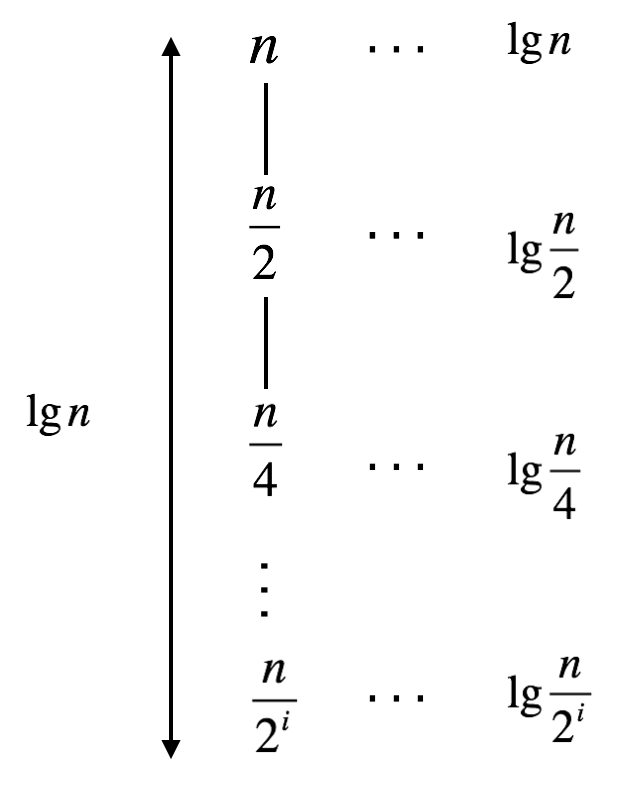
\includegraphics[scale=0.28]{p3b}
	\caption{recursion tree of $B(n)$}
	\label{fig:p3b}
	\end{figure}\\
	The recurrsion tree of $B(n)$ is shown in Figure \ref{fig:p3b}. We get a guess $B(n) = \Theta(lg^2n)$\\\\
	First we prove $B(n) = O(lg^2n)$ part by induction. The inductive hypothesis is $B(\frac{n}{2}) \leq clog^2\frac{n}{2} $ for some constant $c > 0$\\
	Then we have
	\begin{align*}
	B(n) &\leq clog^2\frac{n}{2} + logn\\
	& = c[log^2n - 2logn + 1] + logn\\
	& = clog^2n + c + (1 - 2c)logn\\
	&\leq clog^2n 
	\end{align*}
	\\
	if $c + (1 - 2c)logn \leq 0$. This condition holds when $n \geq 2$ and $c \geq 1$. Thus $B(n) = O(log^2n)$\\\\
	For the lower bound, $B(n) = \Omega(log^2n)$, we use inductive hypothesis that $B(\frac{n}{2}) \geq clog^2\frac{n}{2}$ for some constant $c > 0$\\
	Similarly we have 
	\begin{align*}
	B(n) &\geq clog^2\frac{n}{2} + logn\\
	& = c[log^2n - 2logn + 1] + logn\\
	& = clog^2n + c + (1 - 2c)logn\\
	&\geq clog^2n 
	\end{align*}
	if $c + (1 - 2c)logn \geq 0$. This condition holds when $n \geq 1$ and $c = \frac{1}{4}$. So, $B(n) = \Omega(log^2n)$\\\\
	Thus, $B(n) = O(log^2n)$ and $B(n) = \Omega(log^2n)$. So we conclude that $B(n) = \Theta(log^2n)$

	\item $C(n)=3C(n/2)+nlogn$\\
	We can apply master theorem for $C(n)$\\\\
	$C(n)=3A(n/2)+nlogn$. This is a divid-and-conquer recurrence with $a = 3$, $b = 2$, $f(n) = nlogn$. $n^{log_b a} = n^{log_2 3}$. 
	\\\\Since 
	$$f(n) = \Omega(n^{log_2 3 - \epsilon}), 0 < \epsilon \leq log_2 3 - 1 $$
	Which satisfied the condition in case 1 of master theorem. So $C(n) = \Theta(n^{log_b a}) = \Theta(n^{log_2 3})$\\\\

	\item $F(n)=F(\floor*{logn})+logn$\\
	Since $F(n)=F(\floor*{logn})+logn$, $F(n) = \Omega(logn)$\\
	Dismiss flooring we have
	\begin{align*}
	F(n) &=F(logn)+logn\\
	F(lgn) &= F(lglgn) + lglgn\\
	... &= ...\\
	F(lglg...lgn) &= F(lglg...lglgn) + lglg...lgn
	\end{align*}
	Thus we have:
	\begin{align*}
	F(n) &= lgn + lglgn + lglglgn + ... + lglg...lgn\\
	&\leq clgn, where c = log*(n)
	\end{align*}
	So, $F(n) = O(logn)$.
	Thus, $F(n) = O(logn)$ and $F(n) = \Omega(logn)$. So $F(n) = \Theta(logn)$
\end{enumerate}